\documentclass{beamer}

% === DATOS === (((
\title{Origami, Teselaciones y Teoría de Conjuntos.}
\author{Erick Rodríguez}
\institute{Universidad Autónoma de Aguascalientes.}
% \date{}
% )))

% === PAQUETES === (((
% \usepackage{wasysym}
\usetheme{Warsaw}
\setbeamertemplate{enumerate items}[circle] % esto lo estoy usando para los simbolos de enumeración.
\usepackage{amsfonts}
\usepackage{amsmath}
\usepackage{amssymb}
% \usepackage{expl3}
\usepackage{tikz}
\usepackage{mathrsfs}
\usepackage{graphicx}
% )))

% === TIPOGRAFÍA === (((
\usefonttheme{professionalfonts}
\usefonttheme{serif}
\usepackage{fontspec}
\setmainfont[
  BoldFont       = bodonibi,
	ItalicFont     = Century modern italic2.ttf,
	BoldItalicFont = bodonibi,
	SmallCapsFont  = lmromancaps10-regular.otf
]{Century_modern.ttf}
\setbeamerfont{frametitle}{family=\scshape}
% \usepackage{expl3}
\DeclareSymbolFont{italics}{\encodingdefault}{\rmdefault}{m}{it}
\DeclareSymbolFontAlphabet{\mathit}{italics}
\ExplSyntaxOn
\int_step_inline:nnnn { `A } { 1 } { `Z }
 {  \exp_args:Nf \DeclareMathSymbol{\char_generate:nn{#1}{11}}{\mathalpha}{italics}{#1} }
\int_step_inline:nnnn { `a } { 1 } { `z } {  \exp_args:Nf \DeclareMathSymbol{\char_generate:nn{#1}{11}}{\mathalpha}{italics}{#1}}
\ExplSyntaxOff
% )))

% === COMANDOS === (((
\newcommand{\dis}{\displaystyle}
\renewcommand{\qed}{\hspace{0.5cm}\rule{0.16cm}{0.4cm}}
\newcommand\Myref[1]{
  \begingroup
  \usebeamerfont*{item projected}%
  \usebeamercolor[bg]{item projected}%
  \begin{pgfpicture}{-1ex}{0ex}{1ex}{2ex}
    \pgfpathcircle{\pgfpoint{0pt}{.75ex}}{1.2ex}
    \pgfusepath{fill}
    \pgftext[base]{\color{fg}\ref{#1}}
  \end{pgfpicture}%
  \endgroup
}
\addtobeamertemplate{titleframe}{}{\vspace{-1em}}
% )))

% === COLORS === (((
\beamertemplatenavigationsymbolsempty % for remove the nav. symb.
\mode<presentation>

\definecolor{MSUgreen}{RGB}{216, 90, 55}
% rgb(216, 90, 55)

\setbeamercolor{alerted text}{fg=black}
\setbeamercolor*{palette primary}{fg=white,bg=white!60!MSUgreen}
\setbeamercolor*{palette secondary}{fg=black,bg=white!40!MSUgreen}
\setbeamercolor*{palette tertiary}{bg=black,fg=white!30!MSUgreen}
\setbeamercolor*{palette quaternary}{fg=MSUgreen!10!black,bg=white!05!MSUgreen}

\setbeamercolor*{sidebar}{fg=MSUgreen,bg=MSUgreen!75!white}

\setbeamercolor*{palette sidebar primary}{fg=MSUgreen!10!black}
\setbeamercolor*{palette sidebar secondary}{fg=white!80!blue}
\setbeamercolor*{palette sidebar tertiary}{fg=MSUgreen!50!black}
\setbeamercolor*{palette sidebar quaternary}{fg=white!10!MSUgreen}

\setbeamercolor*{titlelike}{parent=palette primary}
\setbeamercolor{frametitle}{bg=blue!10!MSUgreen}
\setbeamercolor{frametitle right}{bg=white!60!MSUgreen}

\setbeamercolor*{separation line}{}
\setbeamercolor*{fine separation line}{}
\setbeamercolor{block body}{parent=normal text,use=block title,bg=MSUgreen!15!white,fg=black}
\setbeamercolor{block title}{bg=MSUgreen!90!blue,fg=white}

\setbeamercolor{block body example}{parent=normal text,use=block title,bg=MSUgreen!15!white,fg=black}
\mode
<all>
% )))

\begin{document}
\addfontfeature{LetterSpace=-5}

% === PORTADA === (((
\begin{frame}[plain]
	%%%%%%%% Title slide details %%%%%%%%%%%%%%


% Background Image
\newcommand{\myBackround}
{
    
\includegraphics[width=\paperwidth]{IMAGENES/background.png}
}

% Title
\newcommand{\myTitle}
{
	\textsc{Origami, Teselaciones y Teoría de Conjuntos.}
}

% Author
\newcommand{\myAuthor}   
{
    Por Erick Rodríguez.
}

% Affiliation
\newcommand{\myAffiliate}
{
    UAA, LMA.
}

% Presentation Date
\newcommand{\myDate}   
{
    \today
}
%%%%%%%%%%%%%%%%%%%%%%%%%%%%%%%%%%%%


%%%%%%%%%% Title slide code %%%%%%%%%%%
\begin{tikzpicture}[remember picture,overlay]

% Background image
\node[above right,inner sep=0pt] at (current page.south west)
    {
        \myBackround
    };
    
% Title & Subtitle
\node
[
    above=0.5cm,
    align=center,
    fill=orange!10,
    inner xsep=15pt,
    inner ysep=10pt, 
    minimum width=\textwidth,
    text width=0.9\textwidth
] (title) at (current page.center)
{
    \LARGE \myTitle
};

% Author 
\node[ below=0.5cm] (author) at (title.south){\myAuthor};

% Author 
\node[ below=0.1cm] (affiliate) at (author.south){\small \myAffiliate};

% Date
\node[below=0.25cm] (date) at (affiliate.south){\large \myDate};

\end{tikzpicture}

\end{frame}
% )))

% REPASO DE DEFINICIÓN DE ORIGAMI
\section{Definición de Origami y Teselación.} % (((
\begin{frame}[t]
	\begin{exampleblock}{}
		El \textit{origami} (), es el arte japonés de crear superficies de papel a través de realizar \textit{dobleces} a una sola hoja. \\[2mm]
	\end{exampleblock}
\end{frame}

\begin{frame}[t]
	\begin{exampleblock}{}
		Sean \(a < b \) y \(c < d \). Entonces al conjunto \([a,b] \times [c,d] \subseteq \mathbb{R} ^2\) se le llama \textbf{rectángulo}.
		Es decir, un \textbf{origami} es una transformación continua \(T: [a,b] \times [c,d] \longrightarrow \mathbb{R} ^3\), y esperamos que satisfaga lo siguiente.
		\begin{enumerate}
			\item Existe una partición de \([a,b] \times [c,d]\) tal que \(T \big| _{A}\) es inyectiva para cada \(A\) en la partición.
			\item \(T\) preserva ángulos y distancias entre cada par de elementos de un conjunto en la partición.
			\item 
		\end{enumerate}
		Por ser \(T\) continua y \(D\) compacto, \(T(D)\) es compacto.
	\end{exampleblock}
\end{frame}
% )))

% Definición de teselación.
% INTRODUCCIÓN A MANIFOLDS (con animaciones)
% Primer intento de definir doblez (con JM, en triangulos).
% Segundo intento (con alfileres)
% tercer intento (funciones indicadoras) + Teorema
% papers (map foldings) (+ 1 teorema desmotrado)
% intento de definir topología (spoiler resulta la discreta)-

% pi-sistemas
\section{Pi-Sistemas} % (((
\begin{frame}[t]
	\begin{block}{Observación.}
		\begin{minipage}{0.5\linewidth}
			La intersección de rectángulos siempre es un rectángulo. \\[2mm]
			La unión de rectángulos no-necesariamente es rectángulo.
			\[
				\bigg(\dis\bigcup_{i=1}^{n} A_i\bigg) \times \bigg(\dis\bigcup_{i=1}^{m} B_i\bigg) = \dis\bigcup_{i,j = 1}^{n,m} A_i \times B_j.
			\]
			Es decir, no se puede definir una topología cuyos abiertos sólo sean rectángulos.
		\end{minipage}\hspace{5mm}
		\begin{minipage}{0.4\linewidth}
			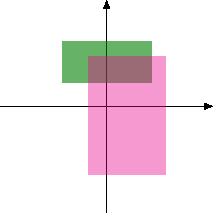
\includegraphics[width= \linewidth, page = 1]{IMAGENES/1_PI_SISTEMAS/1/tikz.pdf}
		\end{minipage}
	\end{block}
\end{frame}

\begin{frame}[t]
	\begin{block}{Definición.}
		Sea \(X \ne \varnothing\). Una colección \(\mathscr{C} \subseteq \mathscr{P}(X)\), es un \textbf{\(\pi\)--sistema} si satisface la siguiente condición.
		\begin{enumerate}
			\item \(\forall A_1, \;\ldots,\; A_n \in \mathscr{C} \;\implies\; \dis\bigcap_{i=1}^{n} A_i \in \mathscr{C}\).
		\end{enumerate}
	\end{block}
	\begin{block}{Lema.}
		Sea \(\mathscr{A}\) conjunto de índices. Si \(\mathscr{C} _\alpha\), \(\alpha \in \mathscr{A}\) es un \(\pi \)--sistema, para todo \(\alpha \in \mathscr{A}\), entonces
		\[
			\dis\bigcap_{\alpha \in \mathscr{A}} \mathscr{C}_\alpha \mbox{ es un } \pi \mbox{--sistema.}
		\]
		\textbf{Demostración.}
		\begin{itemize}
			\item Si \(A_1, \;\ldots,\; A_n \in \dis\bigcap_{\alpha \in \mathscr{A}} \mathscr{C} _\alpha\), entonces
			\item \(A_1, \;\ldots,\; A_n \in \mathscr{C} _\alpha\), \(\forall \alpha \in \mathscr{A}\). Por ser \(\mathscr{C} _\alpha\), \(\pi\)--sistema:
			\item \(\dis\bigcap_{i=1}^{n} A_i \in \mathscr{C} _\alpha\), \(\forall \alpha \in \mathscr{A}\). Por tanto \(\dis\bigcap_{i=1}^{n} A_i \in \dis\bigcap_{\alpha \in \mathscr{A}} \mathscr{C} _\alpha\). \qed
		\end{itemize}
	\end{block}
\end{frame}
% )))

% definir con una operación (algebra).
% Grafos (matriz de adyacencia).

\end{document}
